
\documentclass{article}
\usepackage[utf8]{inputenc}
\usepackage{graphicx}
\usepackage{enumitem}
\usepackage[a4paper,margin=2.5cm]{geometry}
\title{Risposte agli esercizi – Pagina 19}
\author{}
\date{}
\begin{document}
\maketitle

\section*{Esercizio 1}
\begin{enumerate}[label=\textbf{(\arabic*)}]
\item

\begin{center}
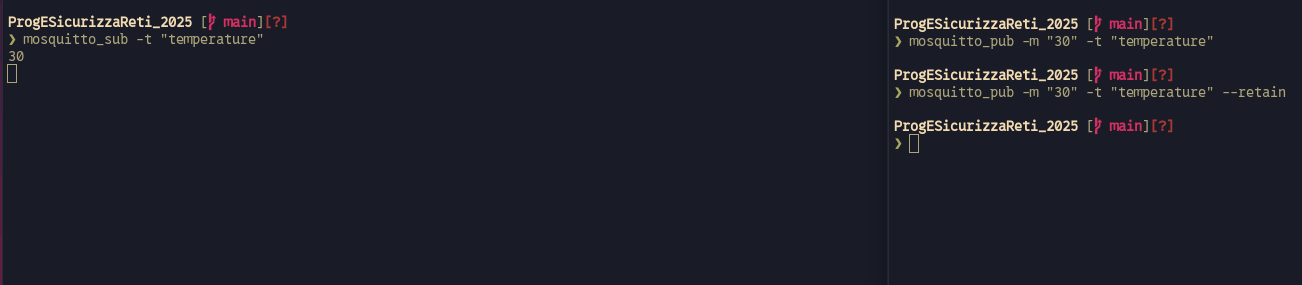
\includegraphics[width=0.8\textwidth]{pub.png}
\end{center}

Come si può vedere il dato viene mandato a vuoto, ovvero sì viene
inviato ma non c'è nessun \emph{subscriber} in ascolto che lo richiede.
Mentre, usando il flag \texttt{--retain}, il dato viene trattenuto
finché non arriva un \emph{subscriber} in ascolto.

\item
Basta un solo terminale per il \emph{publisher}, poiché si invia un
comando alla volta.

\item

\begin{center}
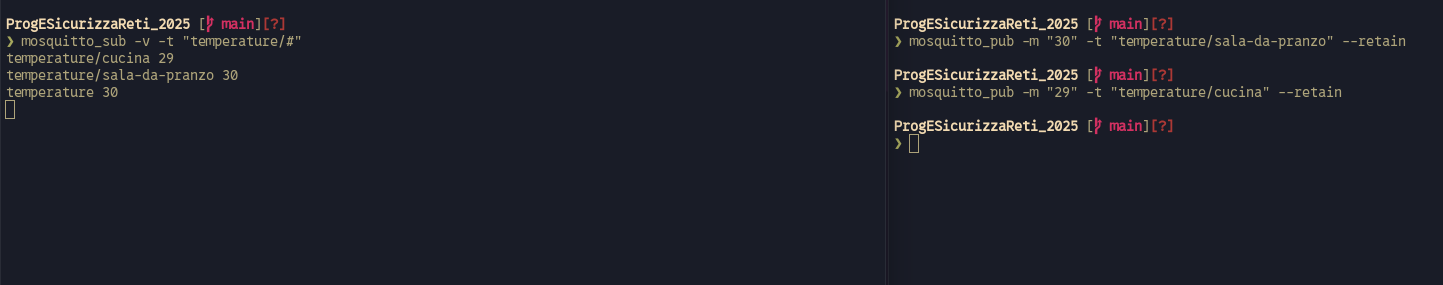
\includegraphics[width=0.8\textwidth]{sub_wildcard.png}
\end{center}

Basta semplicemente utilizzare la \emph{wildcard} \texttt{\#} e
aggiungere l'opzione \texttt{-v} (verbose).

\item

\begin{center}
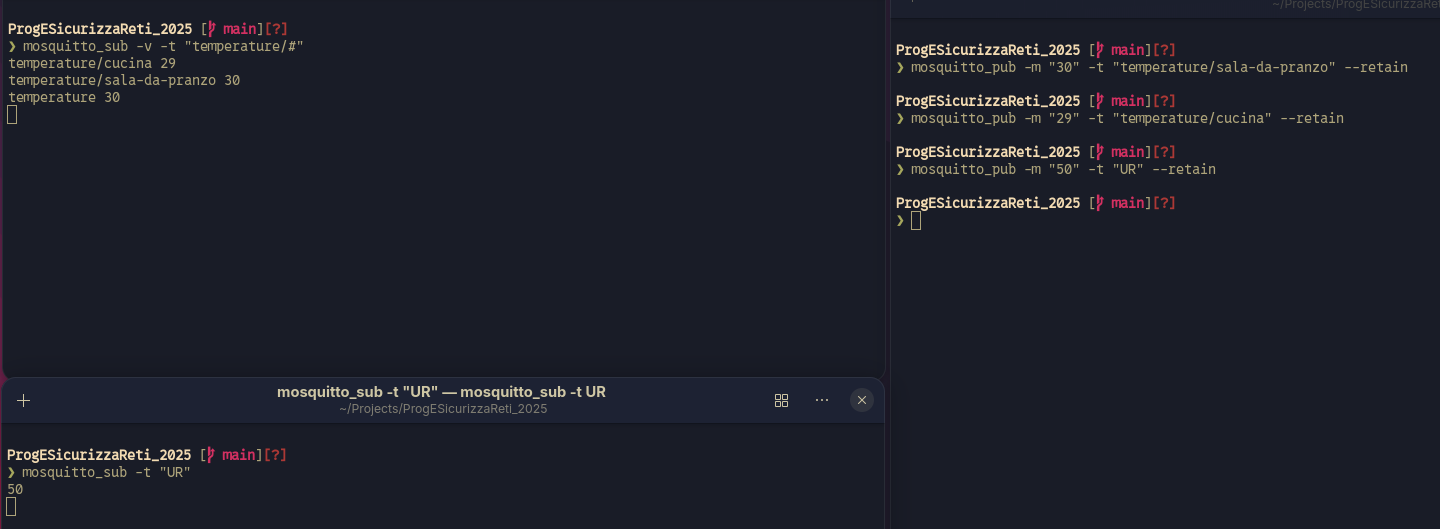
\includegraphics[width=0.8\textwidth]{4term.png}
\end{center}

No, il \emph{subscriber} interessato alle temperature non lo riceve. Si
apre un nuovo terminale e si avvia un nuovo processo \emph{subscriber}
con topic \texttt{UR}.

\item
MQTT utilizza TCP con porta 1883.\\
Il \emph{subscriber} apre una sola connessione verso il broker e rimane
attiva fino al termine del processo. Il \emph{publisher} invece ne apre
una a ogni \emph{publish}.
\end{enumerate}

\end{document}
